%%%%%%%%%%%%%%%%%%%%%%%%%%%%%%%%%%%%%%%%%
% University Assignment Title Page 
% LaTeX Template
% Version 1.0 (27/12/12)
%
% This template has been downloaded from:
% http://www.LaTeXTemplates.com
%
% Original author:
% WikiBooks (http://en.wikibooks.org/wiki/LaTeX/Title_Creation)
%
% License:
% CC BY-NC-SA 3.0 (http://creativecommons.org/licenses/by-nc-sa/3.0/)
% 
% Instructions for using this template:
% This title page is capable of being compiled as is. This is not useful for 
% including it in another document. To do this, you have two options: 
%
% 1) Copy/paste everything between \begin{document} and \end{document} 
% starting at \begin{titlepage} and paste this into another LaTeX file where you 
% want your title page.
% OR
% 2) Remove everything outside the \begin{titlepage} and \end{titlepage} and 
% move this file to the same directory as the LaTeX file you wish to add it to. 
% Then add \input{./title_page_1.tex} to your LaTeX file where you want your
% title page.
%
%%%%%%%%%%%%%%%%%%%%%%%%%%%%%%%%%%%%%%%%%
%\title{Title page with logo}
%----------------------------------------------------------------------------------------
%   PACKAGES AND OTHER DOCUMENT CONFIGURATIONS
%----------------------------------------------------------------------------------------

\documentclass[11pt]{article}
\usepackage[english]{babel}
\usepackage[utf8x]{inputenc}
\usepackage{amsmath}
\usepackage{graphicx}
\usepackage[colorinlistoftodos]{todonotes}
\usepackage{enumitem}
\usepackage{url}
\usepackage{changepage}

\usepackage{tabulary}
\usepackage{caption}
\usepackage{rotating}
\usepackage{tikz}
\usepackage{booktabs}
\usepackage[usestackEOL]{stackengine}
\usepackage{array}
\usepackage{hyperref}
\usepackage{rotating}
\usepackage{wrapfig}
\usepackage{color}
\usepackage{listings}

\begin{document}

\begin{titlepage}

\newcommand{\HRule}{\rule{\linewidth}{0.5mm}} % Defines a new command for the horizontal lines, change thickness here

\center % Center everything on the page
 
%----------------------------------------------------------------------------------------
%   HEADING SECTIONS
%----------------------------------------------------------------------------------------

\textsc{\LARGE University of Twente}\\[1.5cm] % Name of your university/college
\textsc{\Large Project Proposal}\\[0.5cm] % Major heading such as course name

%----------------------------------------------------------------------------------------
%   TITLE SECTION
%----------------------------------------------------------------------------------------

\HRule \\[0.4cm]
{ \huge \bfseries Modelling of Pentago}\\[0.4cm] % Title of your document
\vspace{-1mm}
{ \huge \bfseries using GROOVE}\\[0.4cm] % Title of your document
\HRule \\[1.5cm]
 
%----------------------------------------------------------------------------------------
%   AUTHOR SECTION
%----------------------------------------------------------------------------------------

\begin{minipage}[t]{0.5\linewidth}
%\begin{minipage}{0.4\textwidth}
\begin{flushleft} \large
\emph{Authors:}\\
Theo \textsc{Miltenburg }  -  s0004944\\ % Your name
Wim \textsc{Florijn}   - s1503251\\% Your name
Henk \textsc{Mulder}   - s0169315% Your name
\end{flushleft}
\end{minipage}
~
\begin{minipage}[t]{0.42\linewidth}
%\begin{minipage}{0.4\textwidth}
\begin{flushright} \large
\emph{Supervisor:} \\
Prof. Dr. Arend \\
\textsc{Rensink}% Supervisor's Name
\end{flushright}
\end{minipage}\\[2cm]

% If you don't want a supervisor, uncomment the two lines below and remove the section above
%\Large \emph{Author:}\\
%John \textsc{Smith}\\[3cm] % Your name

%----------------------------------------------------------------------------------------
%   DATE SECTION
%----------------------------------------------------------------------------------------

{\large \today}\\[2cm] % Date, change the \today to a set date if you want to be precise

%----------------------------------------------------------------------------------------
%   LOGO SECTION
%----------------------------------------------------------------------------------------


\includegraphics[scale=0.22]{Images/logo.png} % Include a department/university logo - this will require the graphicx package
 
%----------------------------------------------------------------------------------------

\vfill % Fill the rest of the page with whitespace

\end{titlepage}

\newpage
\tableofcontents
\newpage

\section{Introduction}
\label{Introduction}
Graphs can be used to model various problems.
Behaviour or changes to the modelled system can be expressed using graph transformations.
The changes to this model are a series of graph transformations called rules.
These rules are a three part system: they consist of a left side, a right side and a matching graph.
When the two transformations are executed, from left to right, parts of the graph may be removed and new parts may be added.
This way of modelling graph transformations are called push-outs.
The underlying mechanisms are researched and discussed by Rensink in \cite{Rensink2006}.
This report discusses the modelling of a board game called pentago using such graphs and graph transformations. 
The modeling is done using a tool called GROOVE \cite{tool-groove}.

\vspace{6pt}

Chapter \ref{Pentago} will discuss the game, it's rules and other noteworthy information concerning the playing of the game. 
After discussing the game we will present our model of the game, mayor rules and noteworthy design choices(Chapter \ref{Design}).
We model different strategies, and review their performance in Chapter \ref{Strategy}. Then we draw a conclusion about the results in Chapter \ref{Conclusion}.
Finally, in Chapter \ref{Reflection}, each group member reflects on the course individually.
\section{Pentago}
\label{Pentago}
Pentago is a two-player abstract strategy game invented by Tomas Flodén. 
The company MindtwisterUSA \cite{MindTwisterUSA} has the rights of developing and commercializing the product in North America. %http://www.mindtwisterusa.com/product/classic-wood-pentago


\begin{wrapfigure}{r}{0.5\textwidth}
  \begin{center}
    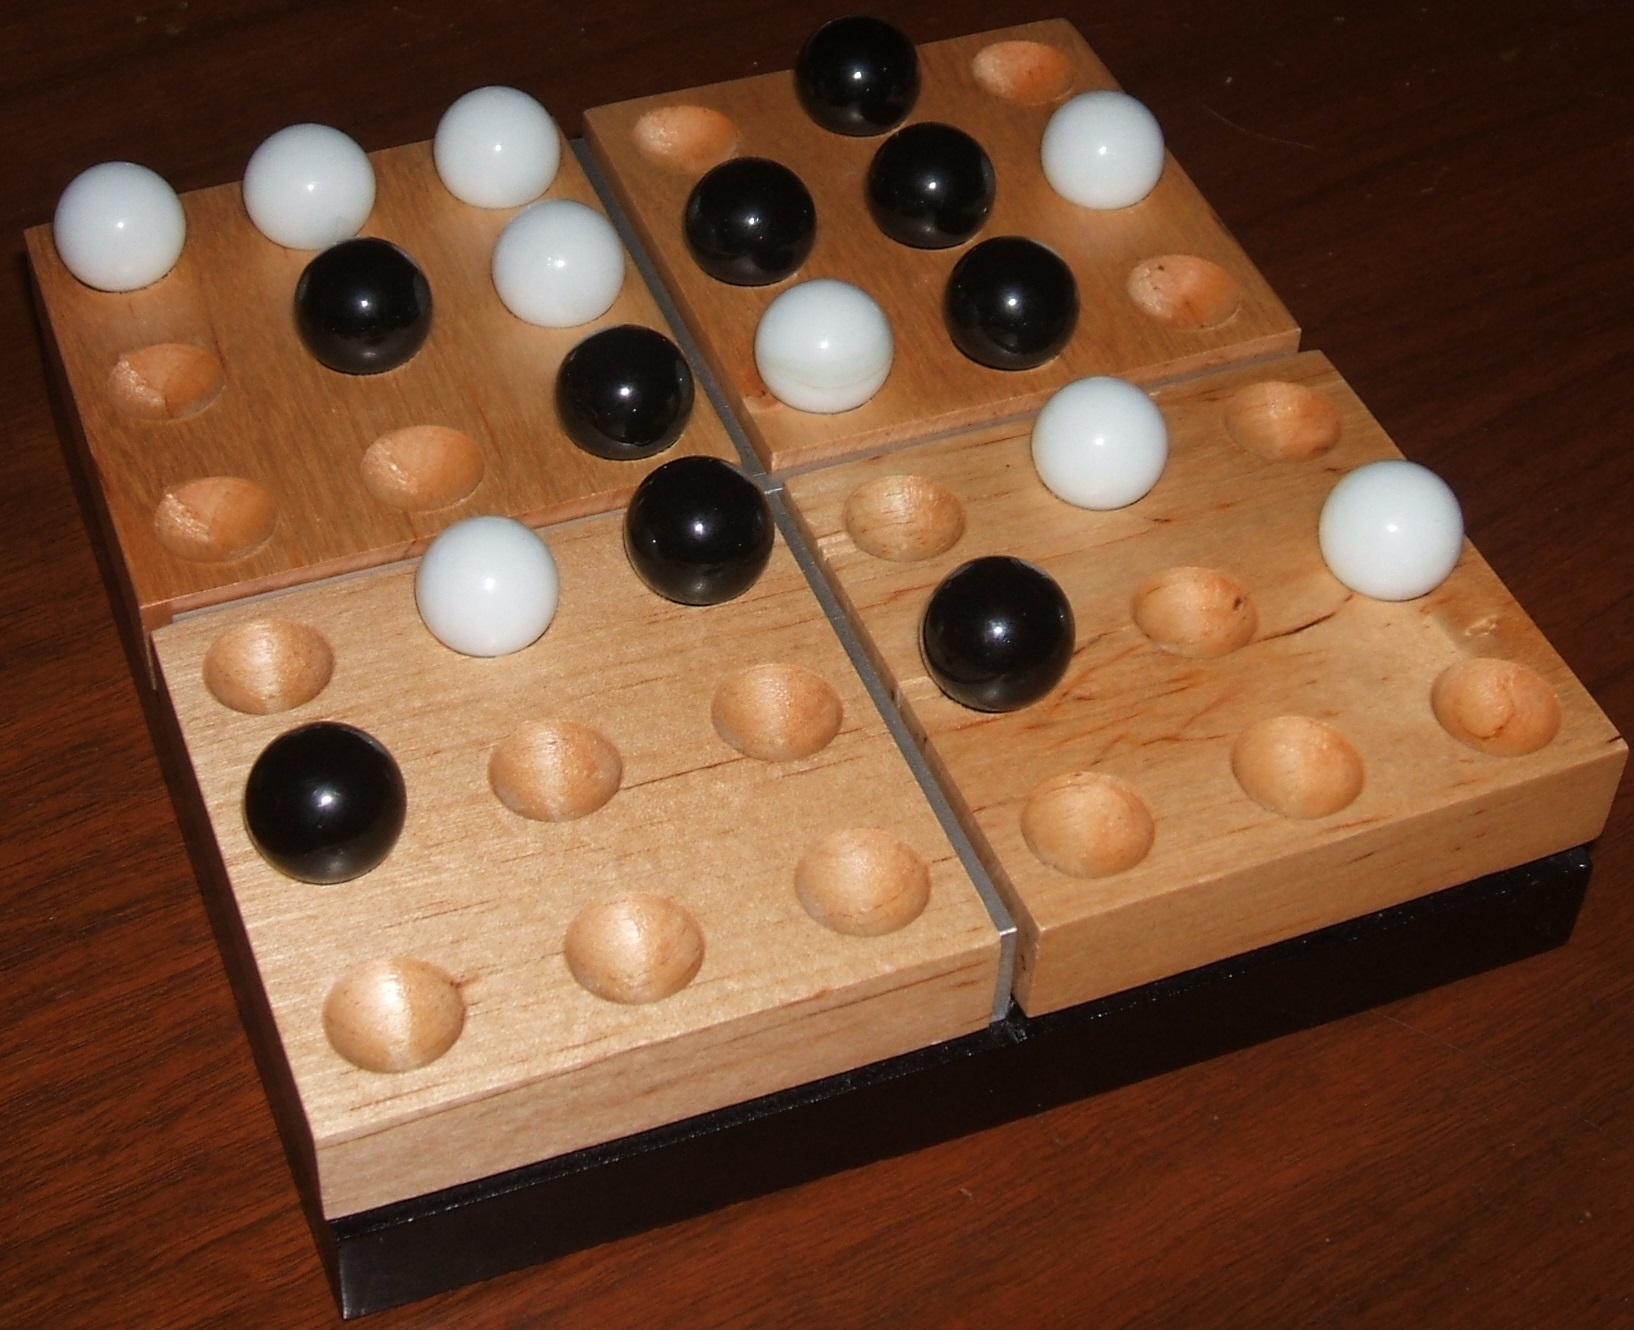
\includegraphics[width=0.48\textwidth]{Images/Pentago-Game-Winning-Position.jpg}
  \end{center}
  \caption{The pentago board}
  \label{fig:boardpic}
\end{wrapfigure}

\vspace{6pt}

Pentago is a two-player game invented by Tomas Flodén. 
The game is played on a 6×6 board divided into four 3×3 sub-boards (also called quadrants). 
Taking turns, the two players place a marble of their color onto an unoccupied space on the board, and then rotate one of the sub-boards by 90 degrees either clockwise or counter-clockwise. 
A player wins by getting five of its marbles in a vertical, horizontal or diagonal row. 
In figure \ref{fig:boardpic} player white wins by possessing a diagonal row. 
If all 36 spaces on the board are occupied without a row of five having formed then the game is a draw.
If multiple players achieve a row of five simultaneously, the game is a draw.
Also a multi-player version for 3 or 4 players has been developed and features a 9×9 board. 
This addition is called super-pentago. 
We plan to model pentago in a scalable fashion so that the board and player size can be defined on initialization.

\section{Model design}
\label{Design}
The game was modeled using different designs. This section will discuss the designs and their up- and down-sides.
The characteristics of GROOVE should be taken into account to optimize the simulation performance. 
In each design the following properties were used:

\begin{itemize}
\item The type "Game" is used to model the the game itself.
\item A type "Player" is used to model a player of the game. The game node features an "currentPlayer" edge to the player whoms turn it is.
\item A type "Space" is used to model a space on the board where a marble can be placed. A marble placement of a player on a space is defined as an "marble" edge from the player node to the space node.
\item An edge "currentPlayer", from the Game to a Player, models whose turn it is.
\item "nextPlayer" Edges between Player nodes indicate the order in which the Players have to play.
\item A "marble" edge from a Player to a Space indicates that a Player has placed a marble on that Space.
\end{itemize}

Also the following rule names were used:

\begin{itemize}
\item "placeMarble": A rule in which the currentPlayer can place a marble on the board.
\item "rotateClockwise" and "rotateCounterClockwise": The rules that model the rotation of a Block on the board.
\item "nextPlayer": The rule that provides the turn-taking mechanism of the palers. The turn taking mechanism has been defined as a graph transformation.
When a player has finished its turn, the currentPlayer edge from the game node is shifted to the player which is connected to by the nextPlayer edge.
The global graph transformation defined for the turn taking mechanism is displayed in figure \ref{fig:turn}.
\end{itemize}

\begin{figure}[!h]
    \centering
    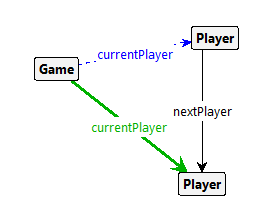
\includegraphics[scale=0.5,clip]{Images/turn.png}
    \caption{Taking turns}
    \label{fig:turn}
\end{figure}

To enforce that the game is played by the rules, a control program has been defined which contains the game flow.
The control program defines the following game flow: As long as possible, a player places a marble, rotates a sub-board and gives the turn to the next player.
The game is finished when a win condition is met, or no marbles can be placed anymore.

\subsection{PentagoXY}
\label{pentagoxy}

The first design modeled the layout of the board by using $x$ and $y$ coordinates for the Spaces where a marble can be placed. 
The board is dynamically generated. The attribute "blocks" determines the size of the board. It indicates the number of blocks in the $x$ and the $y$ direction, with each block being $3*3$ Spaces.
In the start graph there is only one Space node with the coordinates $(0,0)$. Rules were created to create new Spaces in the $x$ and $y$ direction.

A Block on the $x,y$ grid could be identified by the middle Space in the block. Where $x\mod3==1$ and $y\mod3==1$.
Rotating the block was done by changing the coordinate attributes of the Spaces surrounding the middle Space.

\vspace{6pt}

To model the situation where a Player has won, the Direction type was introduced. The Direction node has a $dx$ and a $dy$ attribute.
This way the direction horizontal ($dx=1,dy=0$), vertical ($dx=0,dy=1$) and both diagonal ($dx=1,dy=1$ and $dx=1,dy=-1$) were modeled. 
In the "winner" rule 5 Spaces have to have a marble of the same Player and be spaced repectively $0,1,2,3,4$ times $dx$ and $dy$ for a specific direction.

\vspace{6pt}

This model relies more on attributes than on a graph structure.
The matching strategy of Groove proved to be very inefficient to find a matching for a block. The 9 Space nodes have to be identified by the attributes of the middle space in the block, and the positions relative to these coordinates.
Possible optimizations could be to add flags to the middle space of a Block, and use them to steer the matching strategy of Groove. E.g. to add a flag to the middle Space of the blocks, such that Groove would first try to find these Spaces, instead of trying to find matches for all possible combinations of Spaces.
However it is also possible to add more structure to the graph. 
The extra structure in the model could even convey the intention of the model better to the user, and it might also have better performance in the Groove tool. Therefore a new model of the game was created.

\subsection{PentagoGenerator and Pentago}
\label{pentagoGenerator_and_pentago}

For the second iteration in the development of the model two production systems were created. The "pentagoGenerator" system to generate the board on which to play, and "pentago" to model the actual rules of the game.

\vspace{6pt}

In "pentagoGenerator" a new type named Block is added. This models a $3*3$ block and makes it easier for Groove to match rules to rotate blocks.
The starting graph again consist of a Game node, nodes for the Players and one Block node. From the Game node the first Player is pointed to by the "currentPlayer" edge, and the players are connected by "nextPlayer" edges that model the order in which they can play.
The Game node again has the attribute "blocks", which defines how many blocks the game board has in the $x$ and $y$ direction.

\vspace{6pt}

With the rules "createBlockX" and createBlockY" new Block nodes are created in the respective direction.
With the rule "createBlock" the 9 Spaces of the actual block are created. Again each Space gets an $x$ and $y$ coordinate appointed to it, calculated using the coordinates of the block and the offsets of the spaces within the block.
Within the block are edges that define how "marble" edges need to move when a block is rotated clockwise (cw) or counter-clockwise (ccw).
An entire block including its spaces is visualized in figure  \ref{fig:p2-block}.

\begin{figure}[!h]
    \centering
    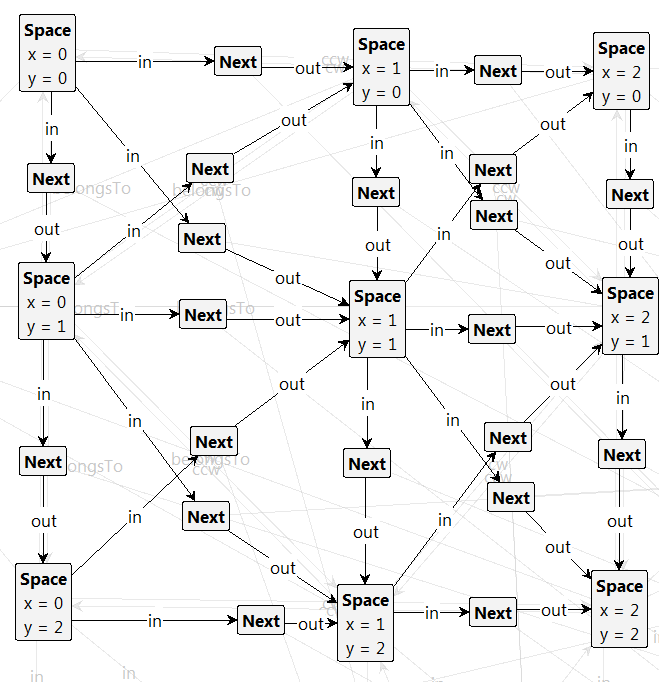
\includegraphics[scale=0.25,clip]{Images/oneblockwithoutbelongs.PNG}
    \caption{A block (sub-board)}
    \label{fig:p2-block}
\end{figure}

\vspace{6pt}

Having 5 marbles in a row is a property that always extends beyond one block.
Therefore the rule "setDirections" is used to dynamically create the structure to model in which directions 5-in-a-row can occur within a block and cross into adjacent blocks.
Again there are 4 Direction nodes in the start graph to represent the directions horizontal ($dx=1,dy=0$), vertical ($dx=0,dy=1$), and both diagonals ($dx=1,dy=1$ and $dx=1,dy=-1$). 
The connection between two spaces is modeled by a Next node that has one "in" edge from the first Space to the Next node, one "out" edge from the Next to the second Space node and a "dir" edge from the Next to the Direction node. This allows to abstract away from the direction in the actual rule to match 5-in-a-row. The connection between two spaces by making use of a direction node is visualized in figure \ref{fig:cspaces}.

\begin{figure}[!h]
    \centering
    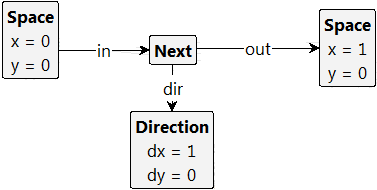
\includegraphics[scale=0.25,clip]{Images/TwoSpacesConnected.PNG}
    \caption{Connected spaces}
    \label{fig:cspaces}
\end{figure}

\vspace{6pt}

In the pentago production system are the rules for the actual game.
It again has the rule "placeMarble" in which the current player can place a marble on the board.

Rotating a block is now done by matching a Block node, and moving all marble edges, from all Players from Spaces that belong to that block, to Spaces that are connected with the direction edge (cw or ccw). The rotation mechanism is visualized in figure \ref{fig:rsb}.

\begin{figure}[!h]
    \centering
    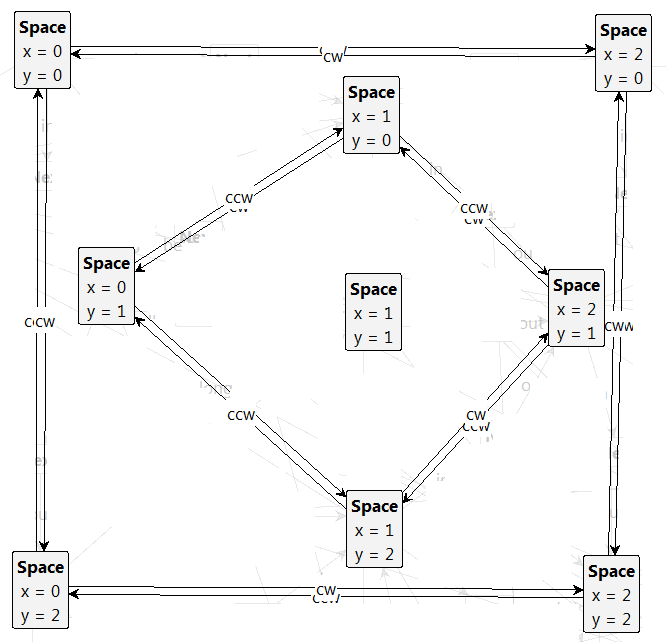
\includegraphics[scale=0.25,clip]{Images/blockforrotation.PNG}
    \caption{Rotating a sub-board}
    \label{fig:rsb}
\end{figure}
\vspace{6pt}

Matching 5-in-a-row is done in the "winner" rule by a rule that matches a Player who has marbles on 5 Spaces that are connected by "in" and "out" edges via Next nodes that are connected to the same Direction node.

In simulation the performance has significantly improved. Rotating blocks is nearly instantaneous. 
However trying to find a match for the "winner" rule takes significant time. 
Finding 5 Spaces out of 36, 4 Next nodes out of 110, 1 Block out of 4 and 1 Player out of 2 with the right connections takes a lot of time if the strategy is not perfect.

\vspace{6pt}

There is more structure in the pentago model than in the pentagoXY model. Dynamically creating the board gives greater flexibility in extending to a multi-player game.
The addition of the Block node nicely captures the notion of the $3*3$ blocks of the game. And as a bonus it also made it a lot better to analyze with Groove.
Using the Next type to abstract away from the directions made it possible to nicely capture the notion of 5-in-a-row for the "winner" rule. However the added complexity in the model also proved to be a bottleneck in analyzing the system.

\subsection{PenagoFinal}

\begin{figure}[!h]
    \centering
    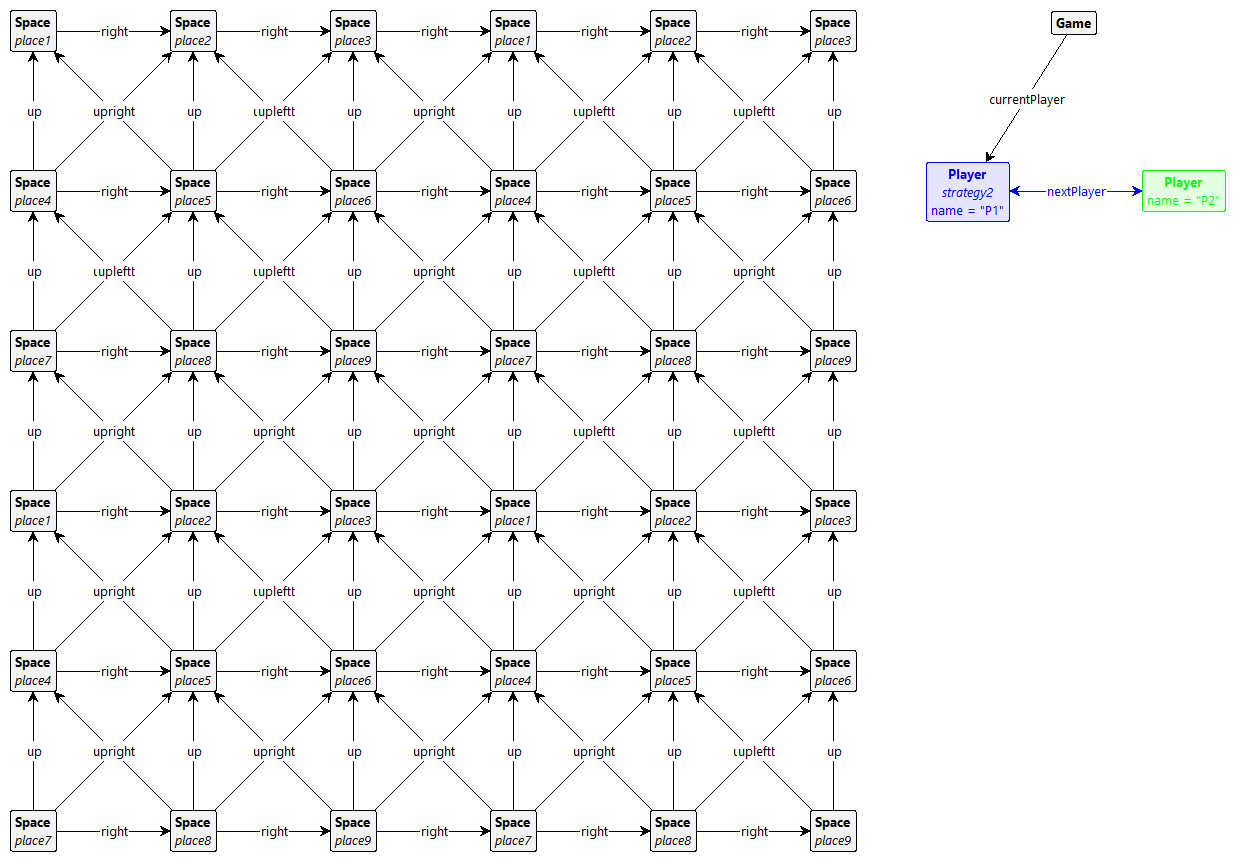
\includegraphics[scale=0.35,clip]{Images/board1.png}
    \caption{Board layout}
    \label{fig:board1}
\end{figure}

This design features 36 spaces in which nodes are connected to their neighbours by horizontal, vertical and diagonal edges.
All spaces in a sub-board hold an unique identifier flag.
The board model is displayed in figure \ref{fig:board1}.

\vspace{6pt}

In this model, the \textit{Game} holds multiple \textit{Players}, which are able to hold multiple \textit{marble} edges to \textit{Spaces}. When the game ends, an edge is created from the \textit{Game} node to a newly created \textit{Finished} node. The full type graph of this model is defined in figure \ref{fig:type_graph_pure_graph}.

\begin{figure}[!h]
    \centering
    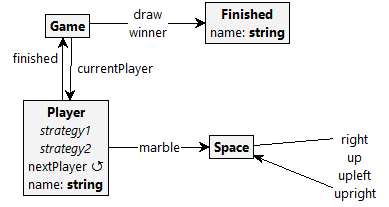
\includegraphics[scale=0.5,clip]{Images/typegraph_puregraphmodel.png}
    \caption{Type graph}
    \label{fig:type_graph_pure_graph}
\end{figure}

\vspace{6pt}

The rotation step in the game flow can be seen as a graph transformation.
In the corresponding graph transformation, the \textit{marble} edges to the nodes on the sub-board are relocated to a clockwise or counter-clockwise node.
This way the board including its connecting edges stay intact.
The graph transformations defined for the rotations are displayed in figure \ref{fig:rotate1}.

\begin{figure}[!h]
    \centering
    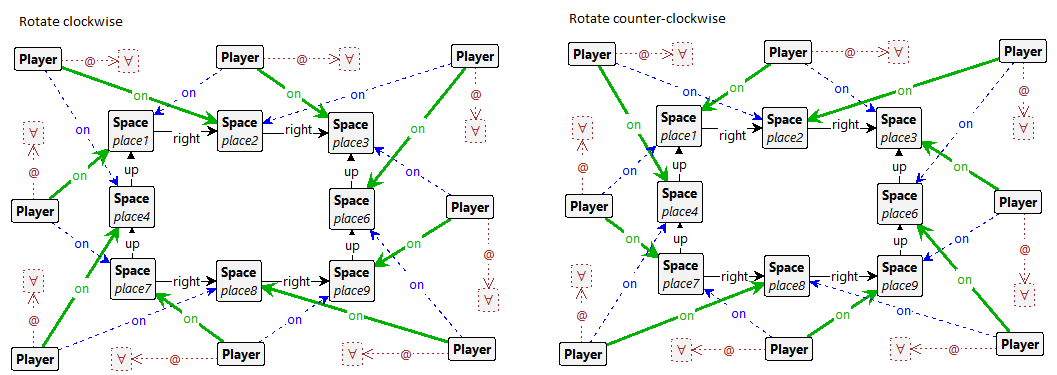
\includegraphics[scale=0.5,clip]{Images/rotate1.png}
    \caption{Rotating a sub-board}
    \label{fig:rotate1}
\end{figure}

\vspace{6pt}

The end-game of pentago is either one player winning the game, or the game ending in a draw.
For a player to win, the player needs to hold \textit{marble} edges to five consecutive nodes.
The game results in a draw when multiple players hold five consecutive nodes simultaniously (this is possible after a rotation), or when no marbles can be placed on the board anymore.

\vspace{6pt}

To check for the winner condition, 4 graph conditions are needed which look whether a row of identical marbles (which are connected by either horizontal, vertical or diagonal edges) exist.
The winner rule which checks for a horizontal row is visualized in figure \ref{fig:endgame1}.
The rules which check for vertical or diagonal rows are identical, except that they check for different edge names.
When a winner rule matches, the \textit{Player(s)} on which the condition matches are connected with a \textit{finished} edge to the \textit{Game}.
The first draw scenario, when multiple players hold a row of consecutive marbles, is achieved when multiple \textit{Players} hold \textit{finished} edges to the \textit{Game} simultaneously.
The draw scenario when no marble can be put on the board anymore, has been defined by using the control program.
When either a winner or a draw is detected, a \textit{winner} or \textit{draw} edge is created between the Game and the Finished node. When a winner is detected, its name is added as an attribute to the \textit{Finished} node. The winner and draw graph condition check for the existence of a \textit{winner} or \textit{draw} edge between \textit{Game} and \textit{Finished}. When it exists the game is finished.

\vspace{6pt}

The seperation of the winning conditions should be seen as a trade-off between scalability and performance: while having 4 individual winning conditions decreases the expandability of the game rules, we have chosen to implement it this way because it decreases the complexity of the computations needed when looking for a winner significantly.

\begin{figure}[!h]
    \centering
    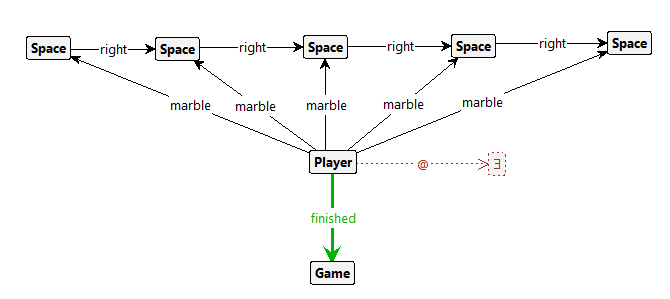
\includegraphics[scale=0.5,clip]{Images/endgame_puregraph.png}
    \caption{Checking for a winner}
    \label{fig:endgame1}
\end{figure}

\vspace{6pt}

While this model is less abstract and thus less scalable than the pentago models described in sections \ref{pentagoGenerator_and_pentago} and \ref{pentagoxy}, the fact that it is a more graph oriented representation makes the model design more clear for users.
Furthermore the usage of edges and node identifiers enable quick matching, which results in a better performance when exploring the state space.
For these reasons this model has been chosen to research smart player strategies.
\section{Strategy}
\label{Strategy}
We find it interesting to research the design of smarter players, who take into account board characteristics when deciding which marble to place or which sub-board to rotate.
There are two players in the game. Each player has a flag if he is employing a specific strategy or plays randomly. 
To compare two players we use a monte carlo style method: We execute a number of playthroughs until one of the final states is achieved (draw or a player wins).
From these playthroughs we gather the execution time, the number of transitions taken and the result of the game.

\vspace{6pt}
\subsection{Algorithm}
The developed strategy is to extend a row of marbles until five in a row has been achieved(and the game is won).
If there is an existing row it will try to extend the longest row.
If there isn't a row,or if there are no rows that can be extended a new row will be started.
 In order to achieve this it has two main rules:
\begin{itemize}
\item Try to extend the longest consecutive row of marbles of its color.
\item Place a marble in a center position
\end{itemize}
Both rules will be discussed in the rules paragraph.
In order to make decisions it first tries to look for a row of 4 marbles and places one marble at either possible end. If this is not available it looks for a row of 3. This pattern repeats till the length of the row is 1.
If it can not find a free Space adjacent to a marble of its own, then it will try to occupy a Space in the center of a block.
If none of the strategy rules can be matched, the system will fall back by placing a marble in a random empty Space.
This algorithm has been implemented in the control program.
Rules and control programs to model the strategy are placed in the "strategy" folder/ package.

\subsubsection{Control Program}

The algorithm  has its own control program in the strategy package to enforce the order in which the rules are matched.
\lstset{ %
	language=C++,                % choose the language of the code
	basicstyle=\footnotesize,       % the size of the fonts that are used for the code
	numbers=left,                   % where to put the line-numbers
	numberstyle=\footnotesize,      % the size of the fonts that are used for the line-numbers
	stepnumber=1,                   % the step between two line-numbers. If it is 1 each line will be numbered
	numbersep=5pt,                  % how far the line-numbers are from the code
	backgroundcolor=\color{white},  % choose the background color. You must add \usepackage{color}
	showspaces=false,               % show spaces adding particular underscores
	showstringspaces=false,         % underline spaces within strings
	showtabs=false,                 % show tabs within strings adding particular underscores
	frame=single,           % adds a frame around the code
	tabsize=2,          % sets default tabsize to 2 spaces
	captionpos=b,           % sets the caption-position to bottom
	breaklines=true,        % sets automatic line breaking
	breakatwhitespace=false,    % sets if automatic breaks should only happen at whitespace
	escapeinside={\%*}{*)}          % if you want to add a comment within your code
}

\begin{lstlisting}
function pm() {
try {
	add2fourLeft|add2fourRight;
}else{
	try{
		add2threeRight|add2threeLeft;
	}else{
		try{
			add2twoLeft|add2twoRight;
		}else{
			try{
			add2oneLeft|add2oneRight;
		}else{
			midBlock;
		}
	}
}
}
}
\end{lstlisting}
The function "pm" (short for place marble) first tries to match one of the rules to extend 4-in-a-row, then for 3 and so on. If no row can be extended the "midBlock" rule  places a marble in the center of a block. If none of these smart rules can be matched a random marble is placed somewhere on a free spot from the main control program.

\vspace{6pt}

To make sure that a player uses its appointed strategy, the "game\_progress" control program in the main package was also updated.
The "executePlace" function first tries to match strategy rules by calling the "pm" function of the strategy. If none of these rules match, either because the player has no strategy flag or because the strategy is exhausted, then it will try to match the general "placeMarble" rule. 

\subsubsection{The rules}
This section describes the special rules which have been composed as part of the strategy.

\begin{figure}[!h]
  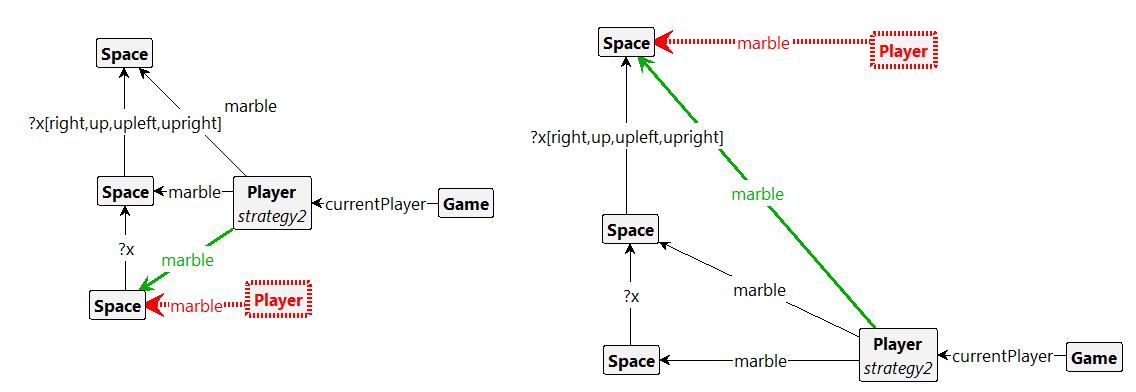
\includegraphics[scale=0.42,clip]{Images/twocombined.png}
  \caption{Two ways of extending a row}
  \label{fig:twocombined}
\end{figure}

The most interesting rule is the extending of an existing row. Edges are one directional, because of this we get two rules for this situation: one for placing a marble at the "beginning" end of the row and one to add to the "end" of the row. Depicted is the rule for extending a row of length 2. Similar rules have been made for rows of length four, three and one.\\
These rows' can be in 4 different directions. To prevent a blowup in the number of rules we chose to use a wildcart for the direction edges, that have to match with "up", "down", "downleft" or "downright".
This does make the matching somewhat slower, since these rules are harder to match. However we feel it is justified because otherwise we would need 4 times the 4 rules to model each direction.

\vspace{6pt}

If there is no existing row to extend, the algorithm tries to place a marble in the center space of a block. This can easily be done by matching on the "place5" flag that is already present on the board. This is done in the "midBlock" rule.

\vspace{6pt}

The algorithm has no strategy for turning sub-boards: there are no additional rules or control programs needed for this part of the game.


\subsection{Results}
To be able to draw a conclusion about whether our strategy performs well, we want to formally evaluate its performance.
Because the game is relatively complex, it is impossible to generate the entire state space of the game, and determine the complete win rate of the naive and the smart strategies.
Therefore we have decided to perform a Monte Carlo simulation. A Monte Carlo simulation produces distributions of possible outcome values.

\vspace{6pt}

We set up an experiment with two players: one that uses the default random strategy, while the other uses the smart strategy. 
Then we execute one random instance of pentago by using the linear-random exploration strategy. This exploration strategy lists all available rule applications, and choses one randomly.
When the game ends, the number of explored transitions, as well as the result (win/draw) and the optional winner are retrieved.
The number of explored transitions indicates how many steps are taken before the game ends.
To perform a covering Monte Carlo simulation, this process is repeated a total of 200 times.

\vspace{6pt}

\begin{figure}[h]
  \centering
  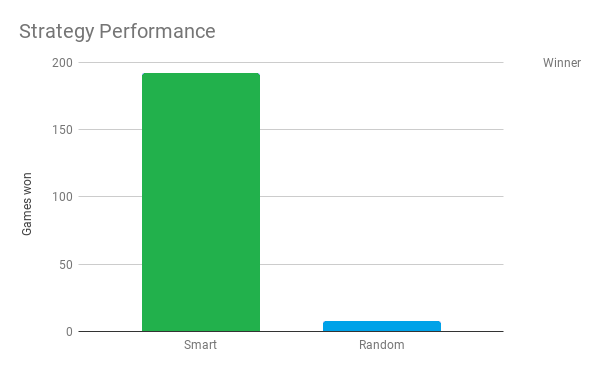
\includegraphics[scale=0.5,clip]{Images/strategywinner}
  \caption{The performance of strategies}
  \label{fig:strategywinner}
\end{figure}

From the results visualized in figure \ref{fig:strategywinner} can be concluded that the random strategy wins only 4\% of the games played. A draw has not occurred in this experiment.
Obviously, there can be concluded that the smart strategy performs significantly better than the random strategy.

\vspace{6pt}

\begin{figure}[h]
  \centering
  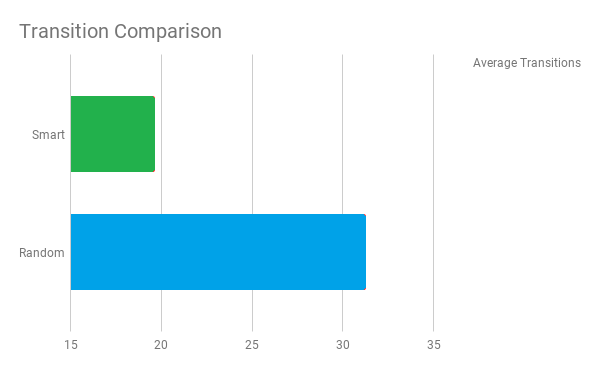
\includegraphics[scale=0.5,clip]{Images/transitions}
  \caption{The number of transitions needed for a strategy}
  \label{fig:transitions}
\end{figure}

From the average transitions can be concluded that the smart strategy finishes the game quicker than the random strategy. Each placeMarble, rotateBoard and nextPlayer rule execution counts as a transition. The smart strategy wins in on average 20 transitions, while the random strategy takes 31 to win. The results are visualized in \ref{fig:transitions}.
\bibliographystyle{unsrt}
\bibliography{refs}

\end{document}